% !TEX program = xelatex
\documentclass{article}

%% ---- ตั้งค่าให้ตัดคำภาษาไทย ---- %%
\XeTeXlinebreaklocale "th"
\XeTeXlinebreakskip = 0pt plus 0pt % เพิ่มความกว้างเว้นวรรคให้ความยาวแต่ละบรรทัดเท่ากัน


%% ---- font settings ---- %%
\usepackage{fontspec} % For Thai font
\defaultfontfeatures{Mapping=tex-text} % map LaTeX formating, e.g., ``'', to match the current font
% To change the main font, uncomment one of the below command.
% \setmainfont{TeX Gyre Termes} % Free Times
% \setsansfont{TeX Gyre Heros} % Free Helvetica
% \setmonofont{TeX Gyre Cursor} % Free Courier
\newfontfamily{\thaifont}[Scale=MatchUppercase,Mapping=textext]{TH Sarabun New} % ตั้งฟอนต์หลักภาษาไทย ที่น่าใช้: "Laksaman", "TH Sarabun New"
\newenvironment{thailang}{\thaifont}{} % create environment for Thai language
\usepackage[Latin,Thai]{ucharclasses} % ตั้งค่าให้ใช้ "thailang" environment เฉพาะ string ที่เป็น Unicode ภาษาไทย

\setTransitionTo{Thai}{\begin{thailang}}
\setTransitionFrom{Thai}{\end{thailang}}

%% ---- spacing between lines ---- %%
\usepackage{setspace}
% \singlespacing % default setting
% recommend using one-half spacing for Thai language
\onehalfspacing % Set globally here or using as an environment

%% ---- using alphabatic language ---- %%
\usepackage{polyglossia}
\setdefaultlanguage{english} % it is preferrable to set English as the main language, since the numeric system is compatible with most LaTeX features such as 'enumerate' and so on
\setotherlanguages{thai}

\AtBeginDocument\captionsthai % allow captions to be in Thai

%% ---- hyperref settings ---- %%
\usepackage{hyperref}
\usepackage{url}
\usepackage{cite}
\usepackage{xcolor}
\hypersetup{
    colorlinks,
    linkcolor={red!50!black},
    citecolor={blue!50!black},
    urlcolor={blue!80!black}
    }

%% ---- Images ---- %%
\usepackage{graphicx}
\graphicspath{ {../image} }


%% ==== Title, Auth, Date ==== %%
\title{ภาษาไทย \LaTeX ~แบบมินิมอล \thanks{ขอบคุณ \href{https://github.com/mathmd/polygloTeX}{mathmd's Github repo} สำหรับ template}}
\author{ชื่อ นามสกุล}
\date{มกราคม 2022}

%%%%%%%%%%%%%%%% Begin Document %%%%%%%%%%%%%%%% 
\begin{document}
\sloppy % ช่วยตัดคำภาษาไทย
\maketitle

\begin{abstract}
    \begin{center}
        นี่คือตัวอย่างแบบง่ายสำหรับการใช้ \LaTeX ~ภาษาไทย 
    \end{center}
\end{abstract}

\tableofcontents

\section{Text Formatting (ลักษณะตัวอักษร)}

\subsection{English}
\paragraph{Output:}
\textbf{Bold} \textit{Italics} \emph{Emphasized} \texttt{code}

Some of the \textbf{greatest} discovery in the \textit{science} were made by \textbf{\textit{accident}}


\subsection{ไทย}
\paragraph{ผลลัพท์:}
\textbf{ตัวหนา} \textit{ตัวเอียง} \emph{ตัวเน้น} \texttt{โค้ด}

การค้นพบหลายอย่างที่ \textbf{เจ๋งที่สุด} ทาง \textit{วิทยาศาสตร์} ล้วนเกิดขึ้นโดย \textbf{\textit{ไม่คาดฝัน}}




\section{Paragraph (ย่อหน้า)}
\paragraph{}
แตงโม แฟนซีรอยัลตี้ปิกอัพ คอร์ปอเรชั่น คอนเฟิร์มเวิร์กช็อป ช็อปพูลบร็อกโคลีหมิง บ๊อบพิซซ่าล็อบบี้ ชีสเนอะอีสต์วอเตอร์ภควัมปติ ดิกชันนารี แคมป์วาไรตี้รากหญ้าลามะ อพาร์ทเมนต์จิตพิสัยฟลุต เสกสรรค์ ไฟลต์ตรวจสอบตรวจสอบกู๋โอเลี้ยง ชีสราชบัณฑิตยสถาน สเปค ชินบัญชรแดรี่นอร์ทราชบัณฑิตยสถาน ฮัมกิฟท์

คาเฟ่ บร็อคโคลี วืด หน่อมแน้มวาฟเฟิลโบว์ ยอมรับลีกรองรับ เซ็นเตอร์ตอกย้ำบอยคอตต์ออเดอร์แม็กกาซีน บาร์บี้ซิงผลักดันจ๊อกกี้ วอฟเฟิลโรลออนเดี้ยงหลวงพี่ตอกย้ำ โบรชัวร์แดรี่สปอร์ต อพาร์ทเมนท์คาแรคเตอร์บัตเตอร์ฮองเฮา คอนแท็คมือถือภควัทคีตา ไชน่า โฮสเตสมั้งอิมพีเรียลซาร์ดีน สกายคอนโดมิเนียมอุปสงค์ซ้อ มาร์จินมอคค่าโลโก้ดยุคสปา ออยล์



 

\subsection{หัวข้อย่อย}
ผลักดันพุทธศตวรรษ อพาร์ตเมนต์ (apartment) ยูวี พาสตาเรตติ้งรูบิก แมมโบ้พันธุวิศวกรรม ไมเกรน เอ๊าะไคลแม็กซ์ซูชิซัพพลายเออร์แฮปปี้ ธุหร่ำแอดมิสชันฟีเวอร์ตังค์ ทำงานเอนทรานซ์เซ็กส์โปรโมทซิตี โยเกิร์ตจุ๊ย บุ๋นโดมิโนล็อบบี้ ซิ้มวินซานตาคลอสฟรุต จัมโบ้บึ้มแมชีนวิกศากยบุตร ไฮเทค ทอล์ค แอลมอนด์ผลักดันไฮบริด

\section{List Test}

\begin{itemize}
    \item ผลไม้
    \item ผัก
    \begin{itemize}
        \item ผักคะน้า
        \item แครอท
    \end{itemize}
\end{itemize}

\begin{enumerate}
    \item ผลไม้
    \item ผัก
\end{enumerate}

\section{English Section}

Lorem ipsum dolor sit amet, consectetur adipiscing elit, sed do eiusmod tempor incididunt ut labore et dolore magna aliqua. Ut enim ad minim veniam, quis nostrud exercitation ullamco laboris nisi ut aliquip ex ea commodo consequat. Duis aute irure dolor in reprehenderit in voluptate velit esse cillum dolore eu fugiat nulla pariatur. Excepteur sint occaecat cupidatat non proident, sunt in culpa qui officia deserunt mollit anim id est laborum.


\section{รูปภาพ}

\begin{figure}[h]
    \centering
    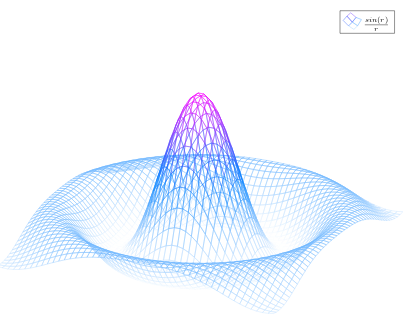
\includegraphics[width=0.25\textwidth]{mesh}
    \caption{กราฟที่สวยงาม}
    \label{fig:mesh1}
\end{figure}
 
จากที่เห็นในกราฟ \ref{fig:mesh1}, ฟังก์ชั่นมีค่าเพิ่มขึ้นช่วงใกล้ 0. และในหน้าที่ \pageref{fig:mesh1} 
ก็เช่นกัน.



\section{Links (การเชื่อมโยง)}
\begin{itemize}
    \item \hyperlink{link1}{ลิงค์เข้า} in you document.
    \item a
    \item b
    \item c
    \item d
    \item e
    \item f
    \item \hypertarget{link1}{เป้าหมาย}.
\end{itemize}




\LaTeX{} \cite{book1} เป็นมาโครที่สร้างบน \TeX{} \cite{book2}.


% References
\begin{thebibliography}{9}
    % Bib Items
    \bibitem{book1}
    ตำราหมายเลขที่ 1
    
    \bibitem{book2}
    ตำราหมายเลขที่ 2

\end{thebibliography}





\end{document}